\documentclass[11pt]{article}
\usepackage{graphicx}
\usepackage{geometry}
\geometry{letterpaper, margin=1in}
\usepackage{caption}
\usepackage{subcaption}
\usepackage{float}

\title{Initial Skewer Analysis at $z=7.4985$}
\author{Aryana}
\date{\today}

\begin{document}

\maketitle

The initial exploratory analysis of the 10,000 sightlines sampled at redshift $z=7.4985$ confirms the geometric and physical validity of the simulation outputs. As shown in Figure \ref{fig:angles}, the probability distributions of the sampling angles ($\cos(\theta)$ and $\phi$) display uniform profiles, verifying that the skewers isotropically sample the unit sphere around the underlying massive halos without directional bias. Moving outward along these sightlines, the 1D density and velocity distributions summarized in Figure \ref{fig:profiles} behave reliably. The individual plotted line-of-sight variations effectively capture stochastic localized structural deviations before smoothly converging toward expected asymptotic mean background values at large distances from the native halo boundaries.

Building upon these physical verifications, Figure \ref{fig:transmission} presents the extracted Lyman-$\alpha$ transmission curves. Most notably, the mean transmission spectrum cleanly illustrates a Gunn-Peterson trough collapsing entirely to zero at wavelengths $<1216$ \AA, accompanied by a prominent damping wing expanding redward. These signatures confirm the overall highly neutral state of the intergalactic medium expected at this redshift.

\begin{figure}[H]
    \centering
    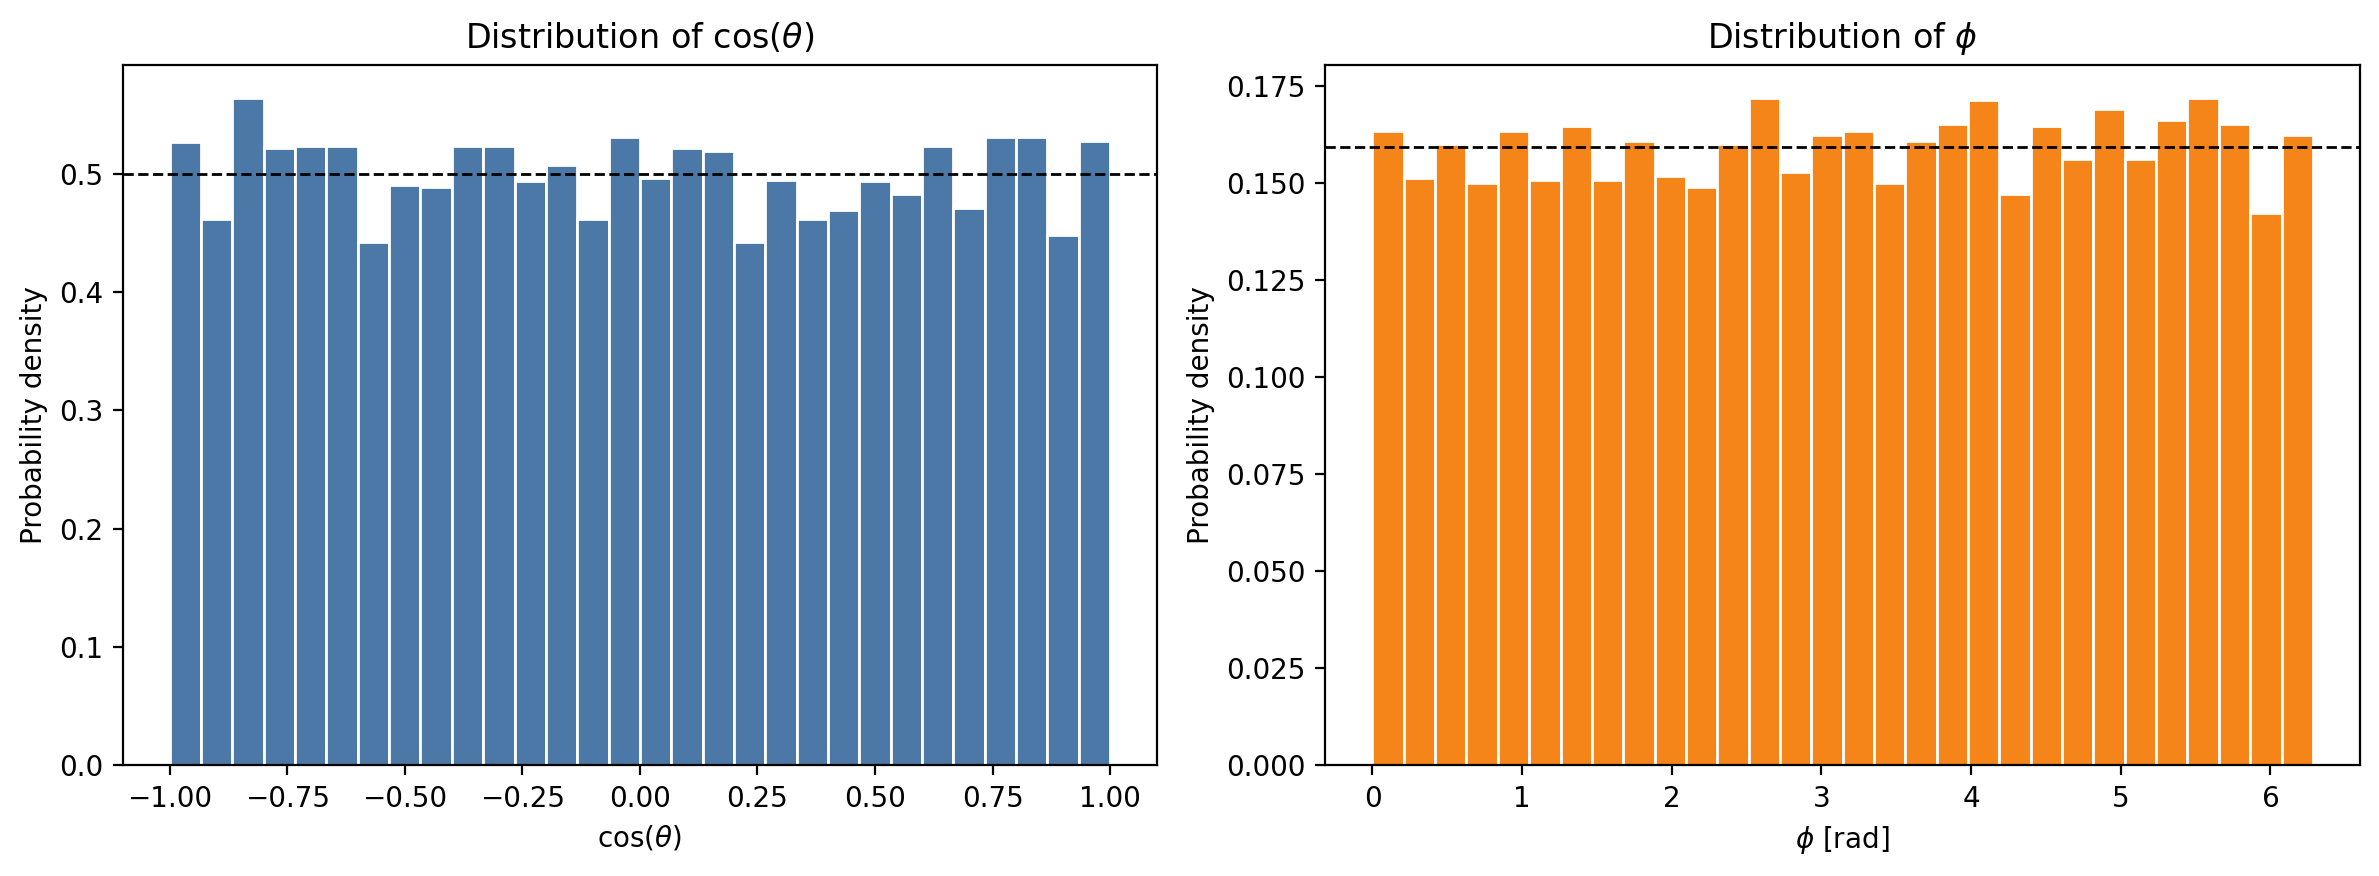
\includegraphics[width=0.8\textwidth]{angle_distributions.png}
    \caption{Probability distributions of the skewer direction angles, demonstrating uniform coverage around the halos.}
    \label{fig:angles}
\end{figure}

\begin{figure}[H]
    \centering
    \begin{subfigure}[b]{0.49\textwidth}
        \centering
        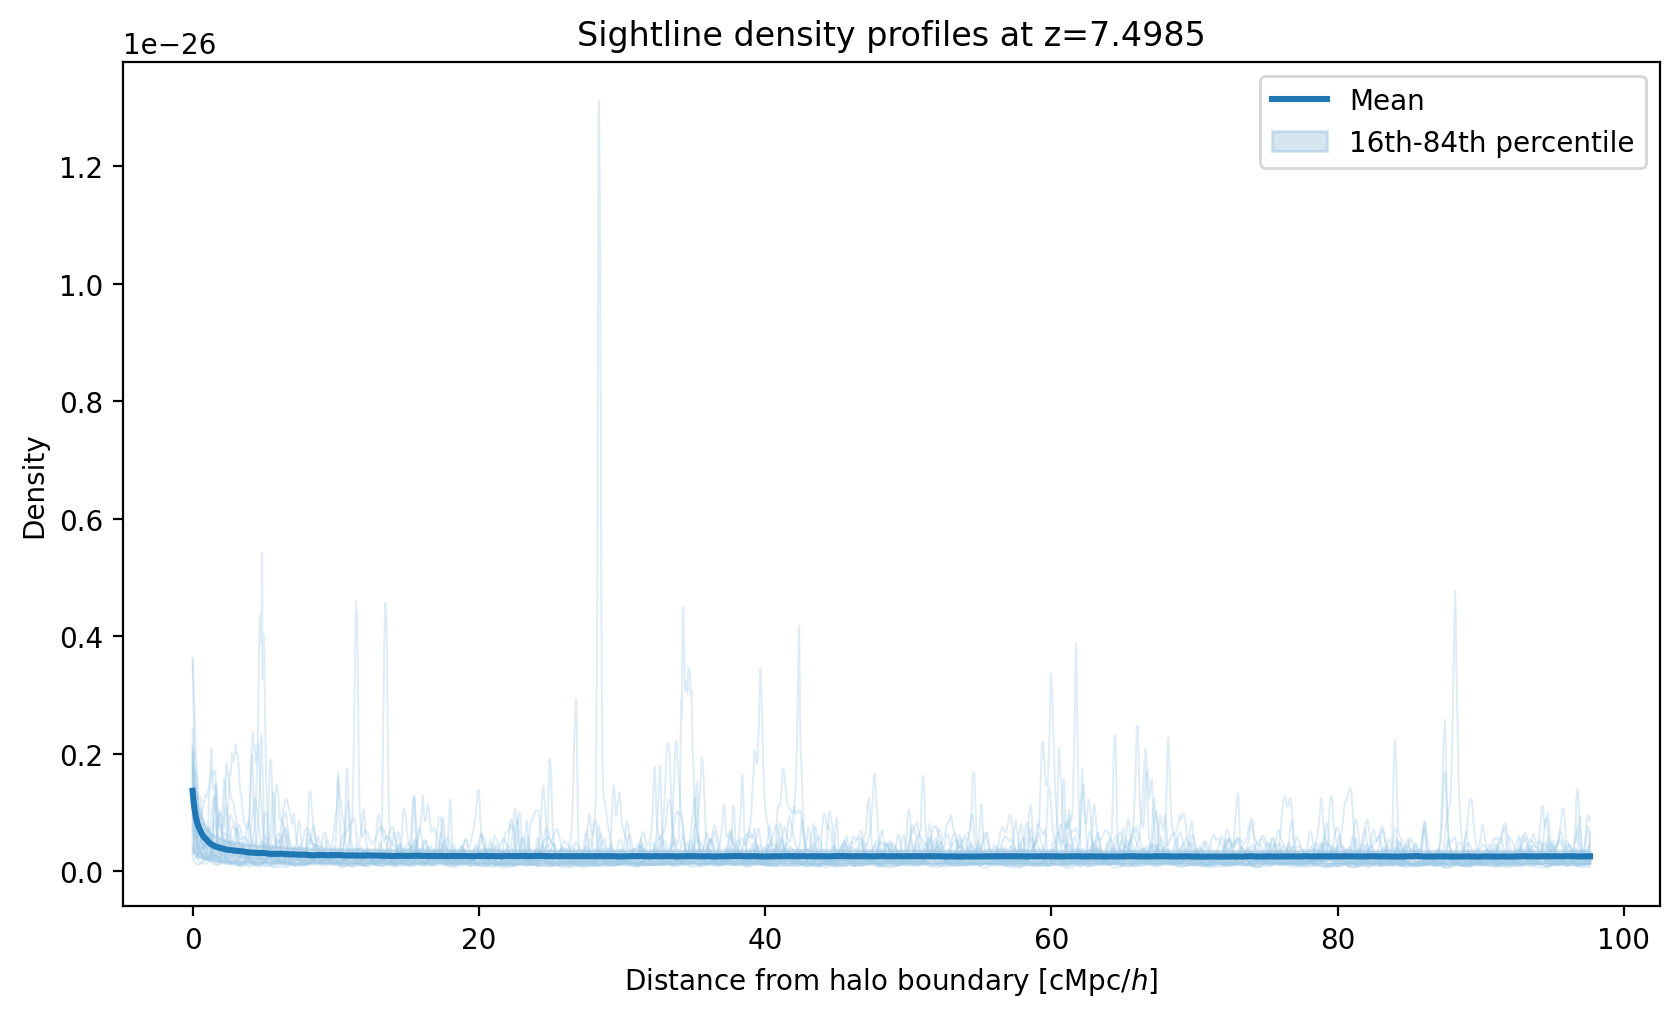
\includegraphics[width=\textwidth]{density_profiles.png}
        \caption{Density Profiles}
    \end{subfigure}
    \hfill
    \begin{subfigure}[b]{0.49\textwidth}
        \centering
        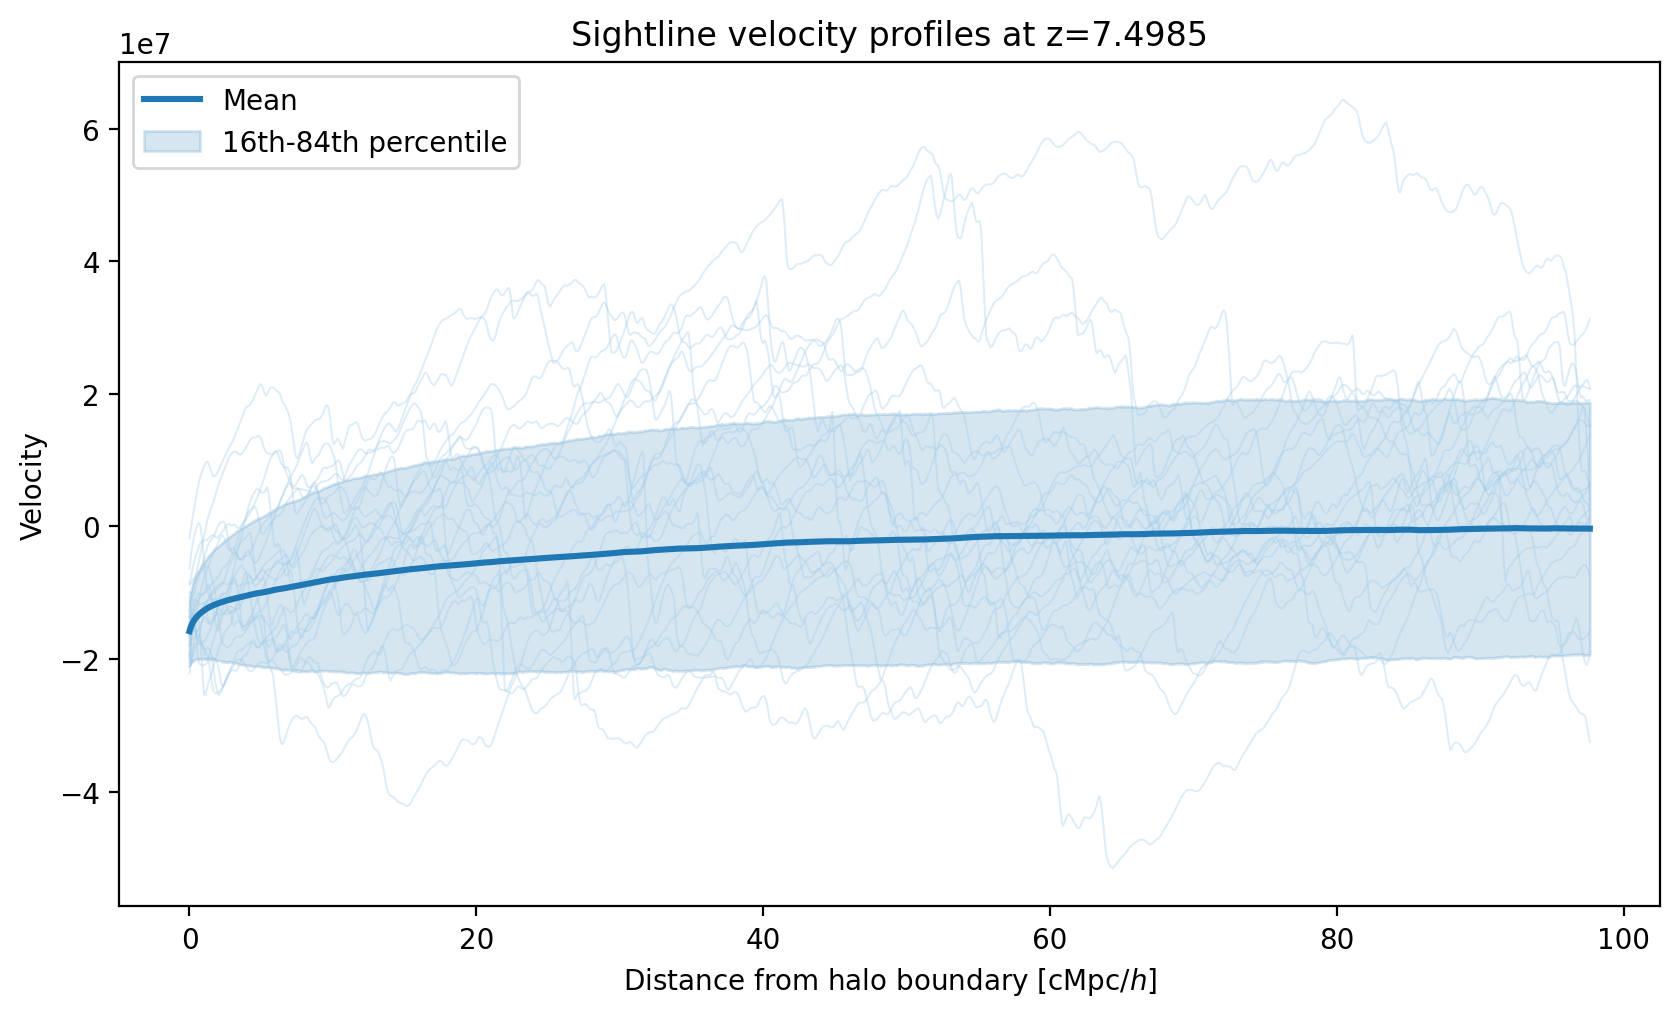
\includegraphics[width=\textwidth]{velocity_profiles.png}
        \caption{Velocity Profiles}
    \end{subfigure}
    \caption{Mean physical quantity profiles extending outward along the sightlines, overlaid with a sample of individual skewers to highlight structural variations.}
    \label{fig:profiles}
\end{figure}

\begin{figure}[H]
    \centering
    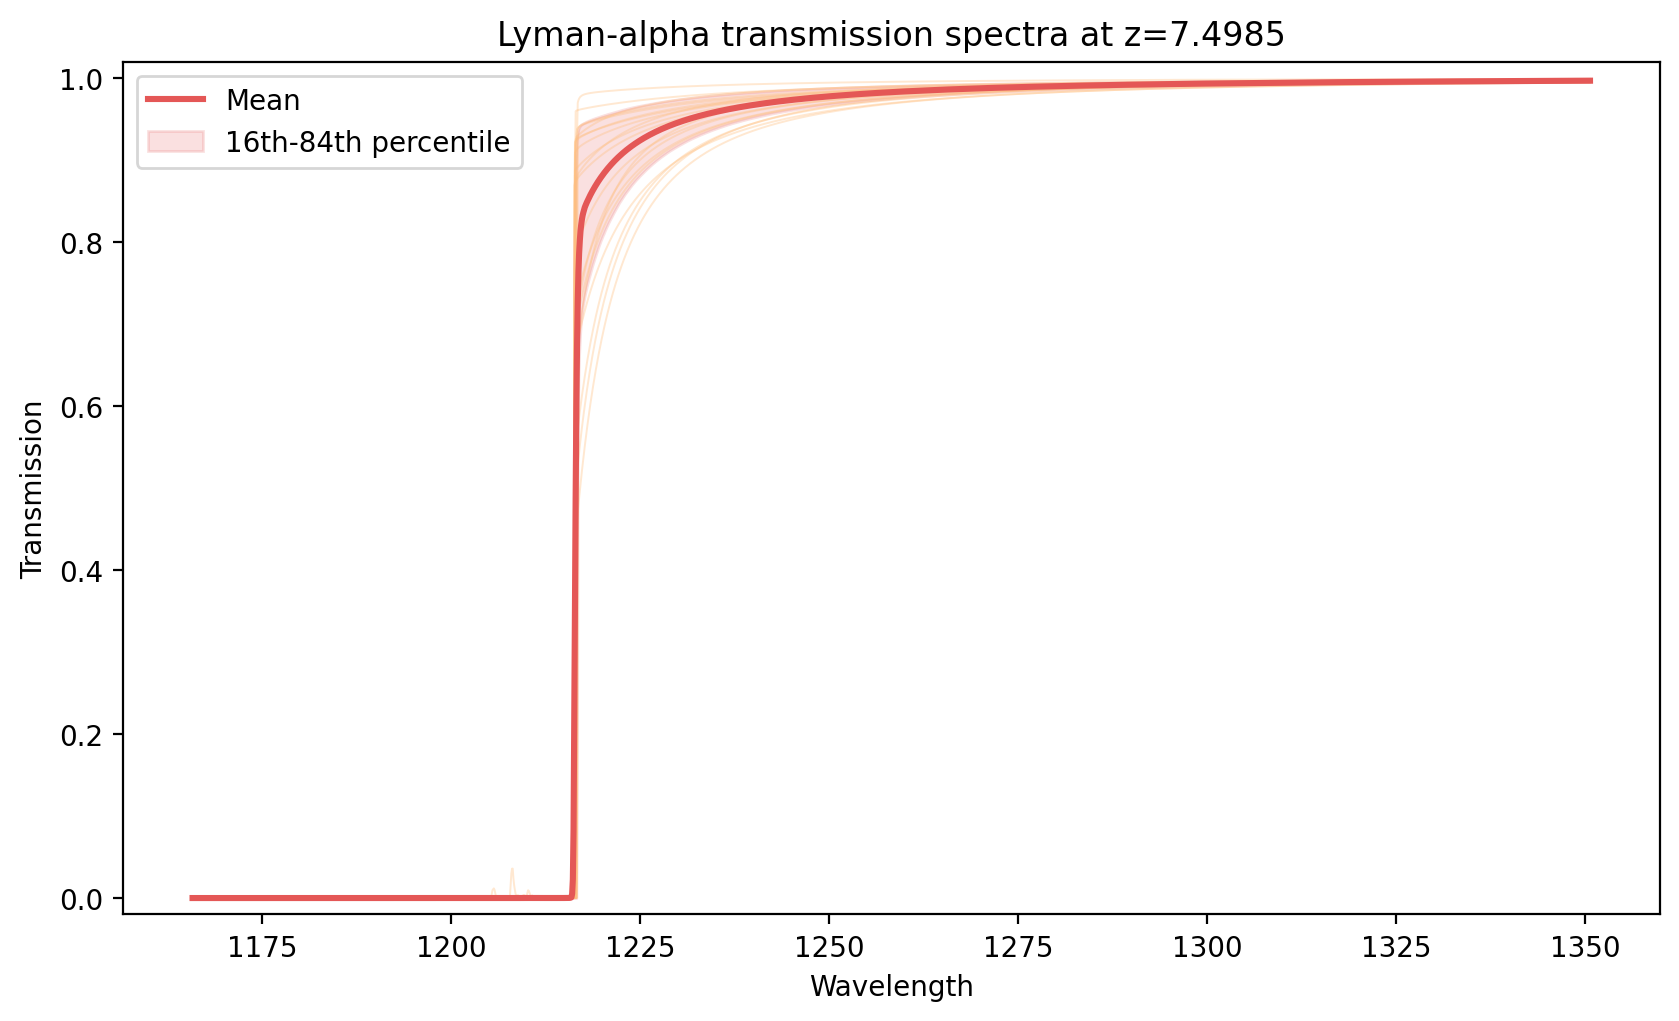
\includegraphics[width=0.8\textwidth]{transmission_spectra.png}
    \caption{Lyman-$\alpha$ transmission curves at $z=7.4985$, heavily exhibiting the Gunn-Peterson trough blueward of the $1216$ \AA \ rest wavelength.}
    \label{fig:transmission}
\end{figure}

\end{document}
